\documentclass[aps,letterpaper,11pt]{revtex4}

\usepackage{graphicx}
\usepackage{float}
\usepackage{verbatim}
\usepackage{amsmath}
\usepackage{amssymb}

\newcommand{\labno}{3}
\newcommand{\labtitle}{Analyzing and Manipulating Data Using Microsoft Excel}
\newcommand{\authorname}{Kevin Truong}
\newcommand{\professor}{Dr. Melanie Lutz}
\newcommand{\classno}{Physics 006}
\newcommand{\labpartners}{Sean Casey, Kevin Castillo, Dulce Payan, and Muhammad Eminic}
\newcommand{\submitdate}{February 14,2017}

\begin{document}

\begin{titlepage}
\begin{center}
\hspace{-136mm}\boxed{{\Large \textsc{Lab No. \labno}}}\\\vspace{30mm}
{\Large \textsc{\labtitle} \\ \vspace{4pt}}
\rule[13pt]{\textwidth}{1pt}\\ \vspace{150pt}
{\large By: \authorname \\ \vspace{10pt}}
Lab Partners: \labpartners \\
Instructor: \professor \vspace{10pt} \\
Solano Community College\\ \classno \\ \vspace{10pt}
\submitdate
\end{center}
\end{titlepage}

\section{Abstract}

Data from a free falling picket fence was collected by the Logger Pro program using a photogate. Organization and manipulation of the collected data was possible with the use of Microsoft Excel. We calculated average velocity and average acceleration with the collected displacements and times. With the collected data and calculated data, we created Displacement vs. Time, Velocity vs. Time, and Acceleration vs. Time graphs. Looking at the linear equation for our linear regression on our velocity vs. time graph, we had an estimation of our acceleration, which was 9.7941$\frac{m}{s^2}$. Our linear regression line on the velocity vs. time graph had an R-squared of 1, which meant that the linear regression was a perfect line. Knowing that the picket fence was in free fall, the acceleration due to gravity should be 9.8$\frac{m}{s^2}$ which is similar to the estimated acceleration obtained. When calculating the percent error, we obtain was 0.06\% error. The disparity between our estimation and the theoretical is possibly attributed to the use of average velocity instead of instantaneous velocity.  

\newpage  

\section{Introduction}

Organizing and manipulating collected data is an important skill that is necessary in reaching a appropriate result. The data we collected in this experiment was from a free falling object(picket fence), therefore we can expect the magnitue of acceleration to be gravity(9.8$\frac{m}{s^2}$). Within this experiment we calculated the average velocity and average acceleration at certain interval of time because a position function wasn't given to be derived for velocity($v = \frac{dx}{dt}$) and subsequently, acceleration($a = \frac{dv}{dt}$). The average velocity equation used in this experiment was $\bar{v_i}=\frac{x_i-x_{i-1}}{t_i-t_{i-1}}$ and the average acceleration equation used in this experiment was $\bar{a_i}=\frac{v_i-v_{i-1}}{t_i-t_{i-1}}$. Percent error is significant in understanding how far off our actual results were from the theoretical results, percent error can be calculated using the equation: $percent\hspace{1mm}error = \frac{|actual - theoretical|}{theoretical}*100\%$. A list of notation used throughout the experiment is presented below; however, these notations will be further articulated throughout the report.   

\begin{center}
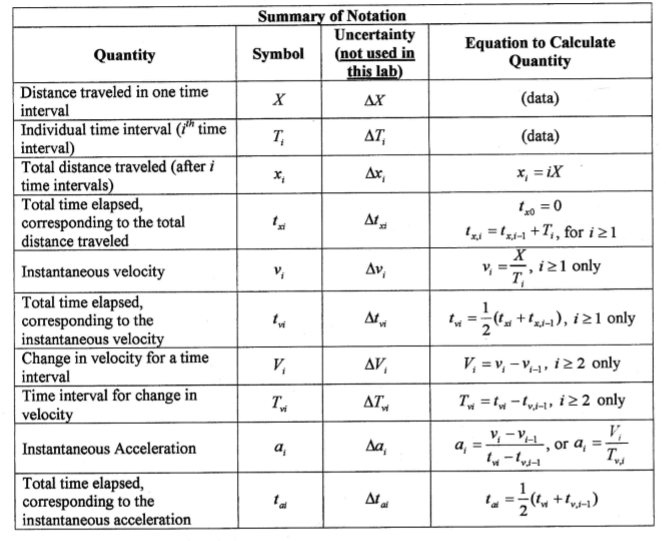
\includegraphics[width=5in]{SummaryOfNotation.png}
\end{center}

\newpage

\section{Experimental Details}

Equipment for this experiment includes a computer, the Logger Pro Program and hardware, an external hard drive, a Vernier photogate, a table clamp, a picket fence, and a landing pad. The computer was used to collect data through Logger Pro, and to manipulate the data received from the experiment within Microsoft Excel. The Logger Pro Program and hardware allowed us to collect and organize the data from the drop in the computer. The external hard drive was used to save the data that we manipulated in Excel.  The Vernier photogate collected the data from the falling picket fence. The table clamp held the photogate in place, so it was sturdy. The free falling picket fence was the object being analyzed, the picket fence had black squares to indicate distance intervals throughout the object. The landing strips was used as a safe landing area for the picket fence, so the picket fence would not break. 

\subsection{The Diagram of Motion Detected by the Photogate}

\begin{center}
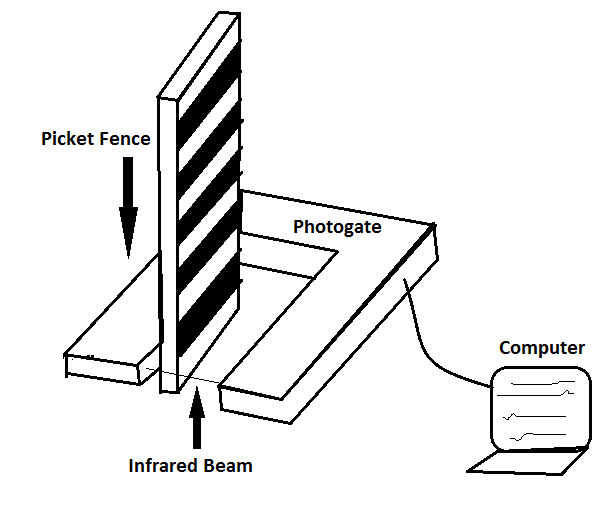
\includegraphics[width=4in]{Setup.png}
\end{center}

When dropping the picket fence, it is important to click "collect" on the Logger Pro program before releasing the picket fence. "Collect" on the Logger Pro program tells the photogate to keep reading until something travels across the sensors. It might be necessary to drop and collect the data from the picket fence multiple times to get nice data. Once all of the necessary data is collected using Logger Pro, all of the manipulation will be made using  Microsoft Excel. Remember to save, periodically, throughout the experiment to avoid the loss of data, in the case that something happens. 



\section{Procedures, Results and Analysis}

\subsection{Taking Time Interval Data}

The data set that we collected and analyzed was from dropping a picket fence through the Vernier photogate. The data from the experiment was the photogate collecting times that the infrared beam hit the opaque parts of the picket fence. After clamping the photogate onto the table to keep it sturdy, opening the shutter on the photogate, placing a landing pad under the photogate to catch the picket fence, and connected the photogate to the computer, we dropped and collected the data from the free falling picket fence; we dropped the picket fence and collected the data about five times until we were satisfied with our data. 

The data was collected through the Logger Pro Program, we had to configure the data collection to photogate by opening a file called 'Motion Timer Picket Fence.cmbl.' To access that file we had traverse through Open-$>$Probes and Sensors-$>$Photogates-$>$Motion Timer Picket Fence.cmbl. After the data collection was configured, we were able to drop and collect the data. The data consisted of sixteen times that were recorded throughout the fall, the time of zero corresponds to the first instance that the photogate is blocked. 

When we were satisfied with the data collected by the photogate, we inserted the external hard drive to save all the necessary files. When saving the initial file, we named the file: "Into to data analysis on Excel" which was cmbl file. A cmbl file is difficult to analyze and manipulate when Logger Pro isn't easily accessable, so the file was exported as a text file into the external hard drive, this file was named "Into to data analysis on ExcelT." Figure 1 is the initial data that was exported into the text file, it is the raw data from the experimental collection.  

\newpage

\begin{center}
Figure 1\\
\vspace{5mm}
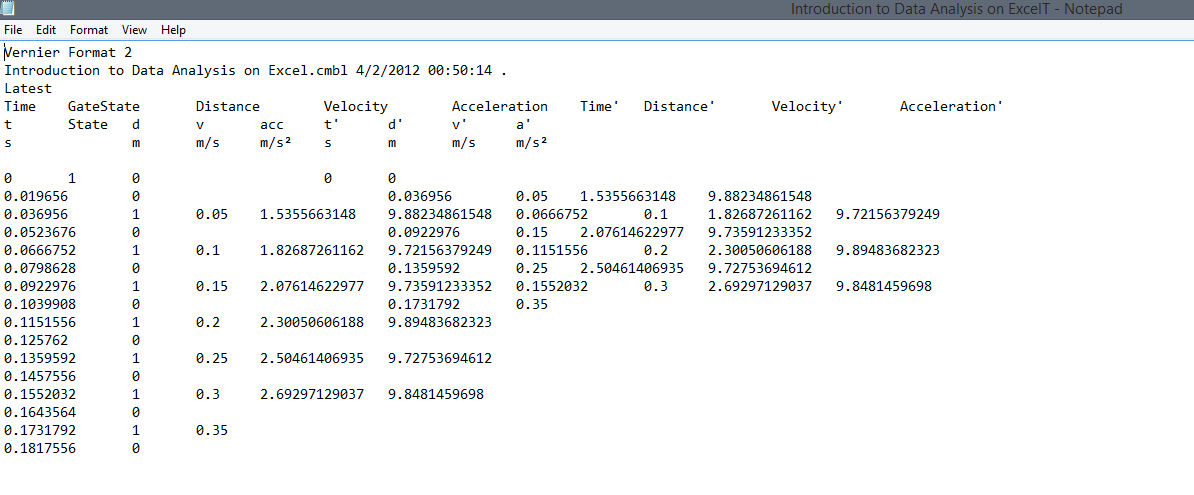
\includegraphics[width=5in]{DataFromCollection.png}\\
\textit{Figure 1: The raw data from the data collection that was exported as a text file from a cmbl file.}
\end{center}


\subsection{Importing the Data into Excel}

\subsubsection{General Tips in Excel}

\begin{center}
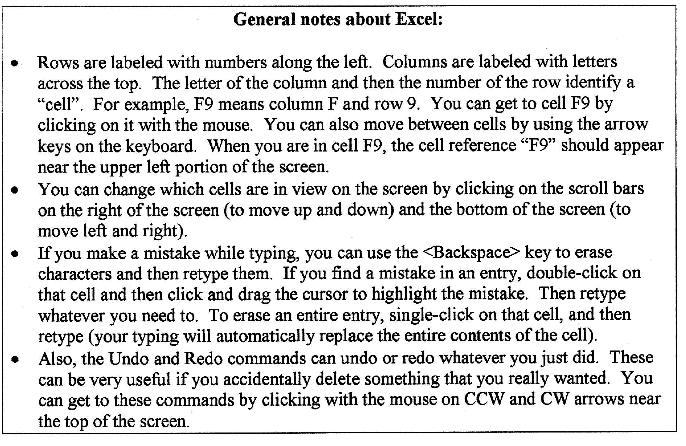
\includegraphics[width=6in]{GeneralNotesExcel.png}
\end{center}

Once the data is exported as a text file, we can import the file into Excel. Within Microsoft Excel, we can import the data of the text file by traversing through Open-$>$My Computer-$>$External Device(drive D). When in drive D, it's necessary to change the "Files of type" box and select "All Files" to see the text file that will be imported. To import the file it was necessary to do the "Text Import Wizard" to import the text file. In the Import Wizard delimited should be checked, and "Tab" should be a delimiter. After the Import Wizard was done running, the data was successfully imported into Microsoft Excel. This Excel file was also saved in the external hard drive as "Intro to data analysis on ExcelE." Once it was saved onto the external hard drive, we were able to press ctrl+s to save the updated Excel spreadsheet. 

We then took all of the data and cut and pasted into cell A50 for formatting purposes and copied all of the raw data(cells A57-A72 and B57-B72) and pasted it into cells B10-B25 and cells C10-C25. We also placed a title heading in cell A1: \textbf{Figure 1: Data Analysis for Picket Fence}. 

\subsection{Distance-Time Calculations}

The data for the time interval was recorded from the instant that the infrared beam on the photogate was blocked once, to the instant it was blocked again by the black bar on the picket fence. The distance from one black bar to the next is denoted by a constant X, the distance is 5cm for each distance of X. The time intervals are from one X to the next X, and are denoted by $T_1$, $T_2$, up to $T_{16}$ where $T_1$ is the first time interval read by the photogate and $T_{16}$ is the last time interval in the experiment. Diagram 1 is the picket fence with X to denote the distance between black squares, and T is the time it takes to travel the distance X. 

\begin{center}
Diagram 1\\
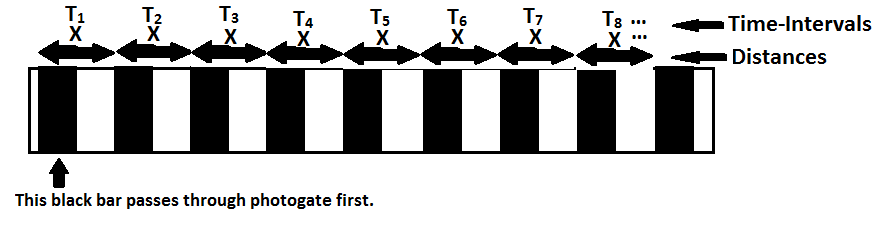
\includegraphics[width = 5in]{TimeIntervalPicketFence.png}\\
\textit{Diagram 1: Diagram of the picket fence showing the constant X distance between each interval.}
\end{center}     

When analyzing the data, the first step is to calculate displacement(x) vs. total elapsed time(t). It's important to note that the x here is lowercase for the displacement and t is lower case for the total elapsed time. While the X in diagram 1 is constant throughout the diagram, the x in diagram 2 is different because it's relative to the starting position which is the initial reading on the picket fence. T in diagram 1 is the time it takes to travel from one X to the next X while t in diagram 2 was the time it took to get to that displacement(x) relative to the start. shows the displacement relative to the start and the time it takes to travel to certain distance. 

\begin{center}
Diagram 2\\
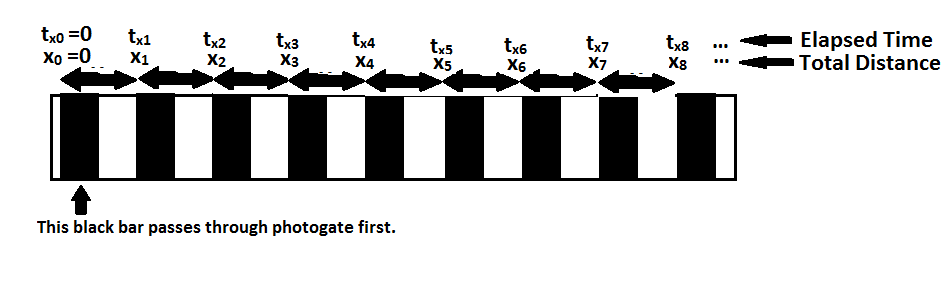
\includegraphics[width = 5in]{ElapsedTimePicketFence.png}\\
\textit{Diagram 2: Diragram of the picket fence showing the displacement relative to the start and the time it takes to travel from the start to a specific displacement.}
\end{center} 

We are only interested in the times that the black squares block the infrared beam, so we deleted any row in column C with a zero. A zero in column C indicated the time interval that the infrared beam wasn't blocked by a black square, and a one indicates the time interval that the infrared beam was blocked. Once we deleted the rows that correspond to the time interval whence the beam wasn't blocked, we can delete all of the ones in column C to only keep the time intervals corresponding to the deleted ones. Then we labeled column A zero to seven to correspond with the displacement of 5cm when the infrared beam was blocked by the black square. 

Row 9 was the headings for each column. In cell A9 we placed a heading of \textbf{i}, and it was used as a counter. The heading for column B was \textbf{L P Time (s)}, for the times collected in Logger Pro. The heading for column C was \textbf{$T_i$ (s)} for the time intervals. We generated the time intervals in column C by typing in the equation: "$= \textbf{B11-B10}$" into cell C11. The number that was generated in C11 was the collected time differences between each increment of collected time. We then copied that same formula down by clicking the desired cell and dragging the green solid box down to C17, all of the cell references changed automatically. 

Columns D and E were used for total time elapsed and total displacements, respectively. The heading for column D and E were {$t_{xi} (s)$ and $x_i (m)$, respectively. Cell D4 was just used as format and the text was \textbf{X (m)}= and in E4 the value placed was \textbf{0.050} for the distance between each interval which is 0.050m. 

The calculations for column D was accomplished by putting zero in cell D10, and the equation =\textbf{D10+C11} in cell D11. This adds the value of D10 and C11 and places the sum in D11. To do the same calculations for all of column D, we dragged the desired cell down to D17. 

To calculate the displacement for column E, we have to use the distance between black squares which is 0.05m and multiply this by the increments in column A. However, we wanted the 0.05m to be static when dragging the equation down for all of column E we had to put "\$" between the cell that we wanted to represent the 0.05m, which was cell E4. The final equation that we had to use in cell E10 to allow us to drag down without any problems was =\textbf{A10*\$E\$4}. 

\subsection{Distance-Time Graph}

After we manipulated our data to obtain the desired data. We graphed all of the data, to create a distance vs. time graph. We created the graph by clicking and dragging the desired cells to be graphed(D9 to E17 which is the time and displacement columns), so the cells were highlighted and clicked "insert" on the toolbar and then chose the "Scatter" chart that only had points. We also added "Axis Titles" and "Legend" by clicking the "Chart Elements" on the graph. We named the graph: \textbf{Figure 3: Displacement Vs. Time}. We also changed the names of the x-axis to be Time (s) and the y-axis to be Displacement (m). We dragged the graph to are that spanned between cells A20 and E37 to have the graph in a nice viewable place. 

It was also necessary to have a caption on the graph, so we added a textbox under "Insert" on the toolbar onto our displacement vs. time graph. The caption that we placed onto the graph was: "This Graph shows displacement vs. time of the picket fence in free fall. It's parabolic inidcating a constant acceleration." We also resized it to fit niceley onto the graph without blocking anything important.  

\begin{center}
\textit{Finished Displacement Vs. Time Graph}\\
\vspace{-15mm}
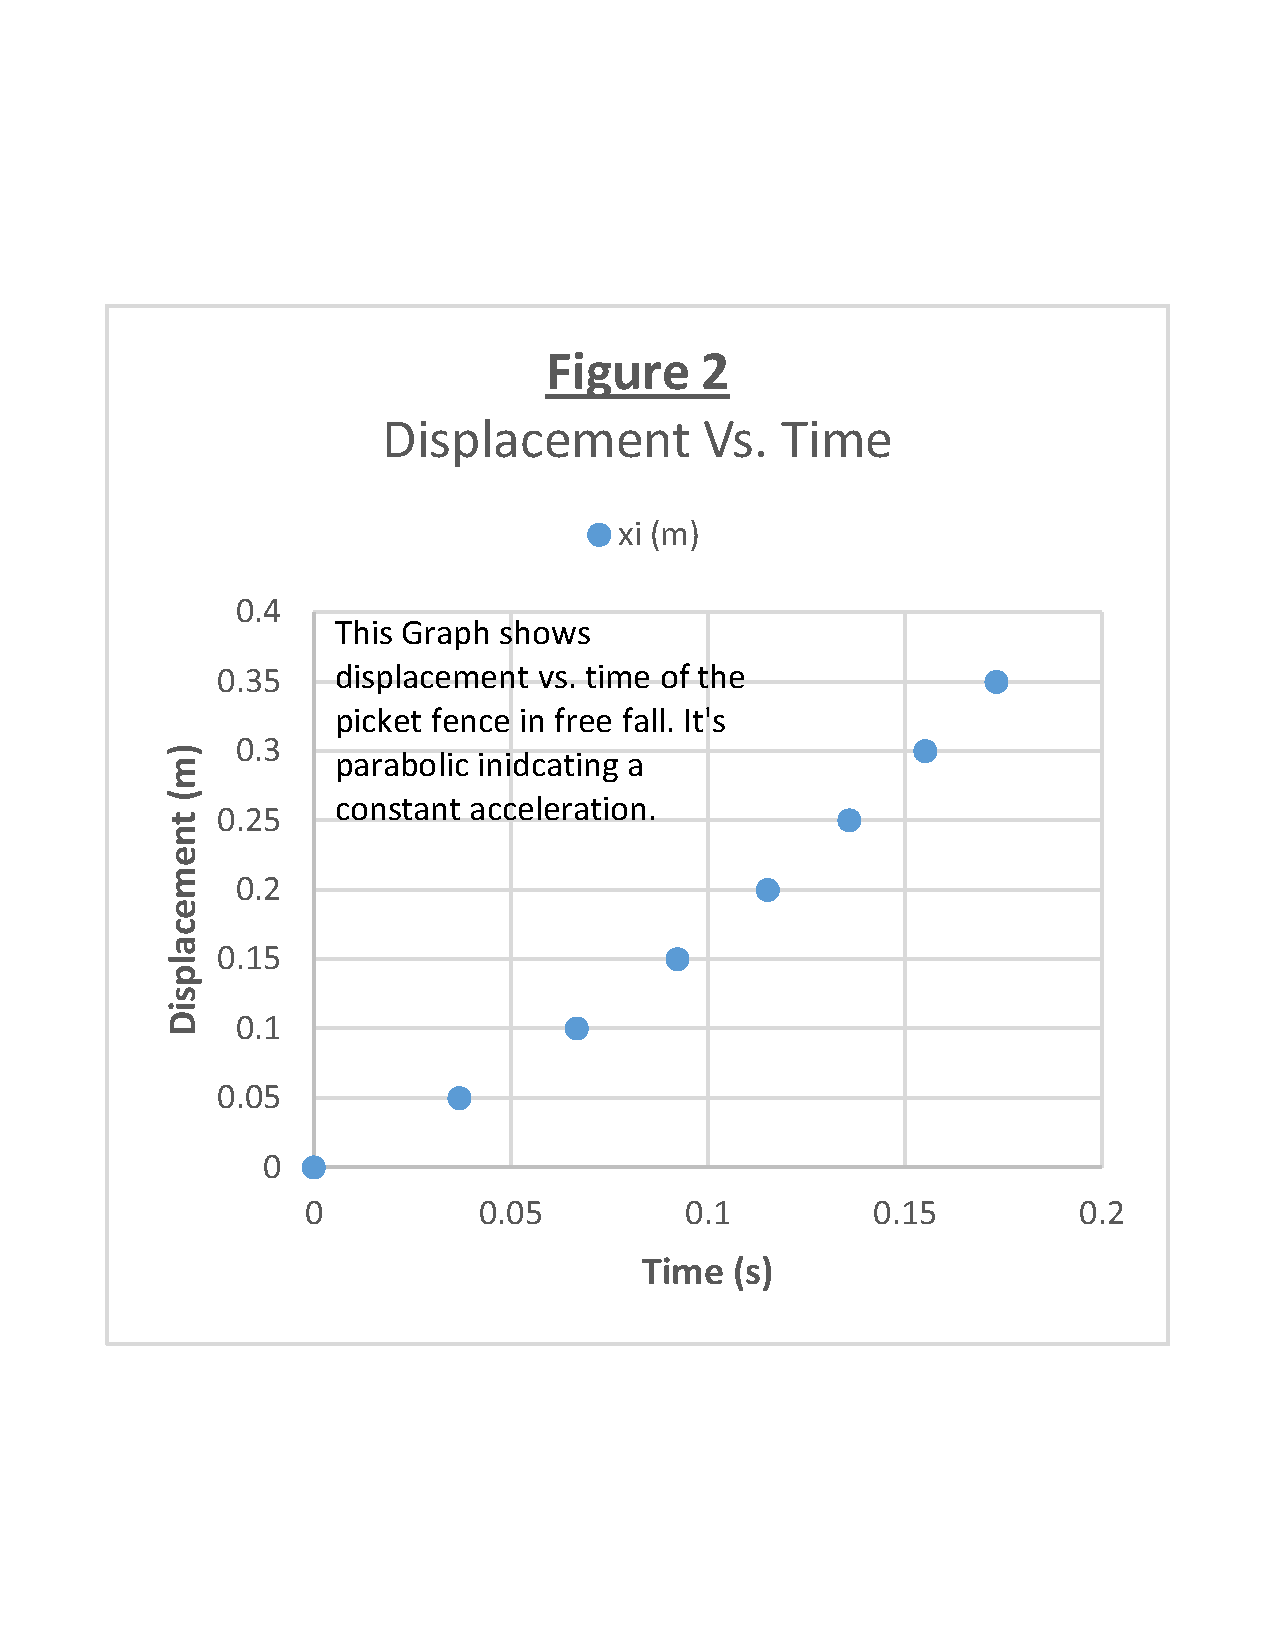
\includegraphics[width=3.5in]{DisplacementVsTimeGraph.pdf}
\end{center}    
 
 \vspace{-20mm}
\subsection{Velocity-Time Calculations}

Since we don't have a function for displacement that can just be derived to obtain instantaneous velocity, it's necessary to estimate the instantaneous velocity values by calculating the average velocity values. Average velocity can be calculated with the equation $\bar{v_i} = \frac{x_i - x_{i-1}}{t_{xi} - t_{xi-1}}$ or simpler $v_i = \frac{X}{T_i}$; however, using this method it's not possible to calculate $v_0$. To calculate a good estimate for the time instant that corresponds to $v_i$, we have to say that $v_i$ is the velocity at the time between time instances $t_{xi}$ and $t_{xi-1}$. To find this time that corresponds to $v_i$, we have to use the equation $t_{vi} = \frac{1}{2}(t_{xi}+t_{xi-1})$. 

In cell G9 and H9, we entered the column heading \textbf{$t_{vi} (s)$} and \textbf{$v_{i} (m/s)$}, respectively. Since it wasn't possible to calculate $v_0$, cells G10 and H10 are left blank. In cell G11 we calculated the value for $t_{v1}$ by using the equation "=0.5*(D11+D10)" or the using the equation mentioned earlier: $t_{v1}=\frac{1}{2}(t_{x1}+t_{x0})$. We copied the same equation down column G by dragging the cell with the desired equation to G17. 

The average velocity for each instant was placed in column H. We started by typing the equation "=(E11-E10)/(D11-D10)" or $\bar{v_1}=\frac{x_1-x_0}{t_{x1}-t_{x0}}$ in cell H11. This equation was copied down colum H, to get the remaining average velocities. Then we created a Velocity vs. Time graph and gave the graph a title, axis titles, and a caption using a text box from "insert." Once we satisfied the requirements, we dragged the graph next to the Displacement vs. Time graph.

\subsection{Slope of Velocity-Time Graph: Experimental Value of Acceleration}

To estimate the acceleration for this experiment, we look at the best-fit slope of the velocity vs. time graph. The linear regression function in Excel allowed us to obtain the best slope for our line. To obtain the regression line we traversed through Layout-$>$Trendline-$>$Linear. We also displayed the linear equation for the line and the R-squared value, by going to More Trendline Options and then checking the boxes "Display equation on chart" and "Display R-squared value on chart." Figure 3 shows the finished Velocity vs. Time graph that we created.

\newpage

\begin{center}
\textit{Finished Velocity Vs. Time Graph}\\
\vspace{-10mm}
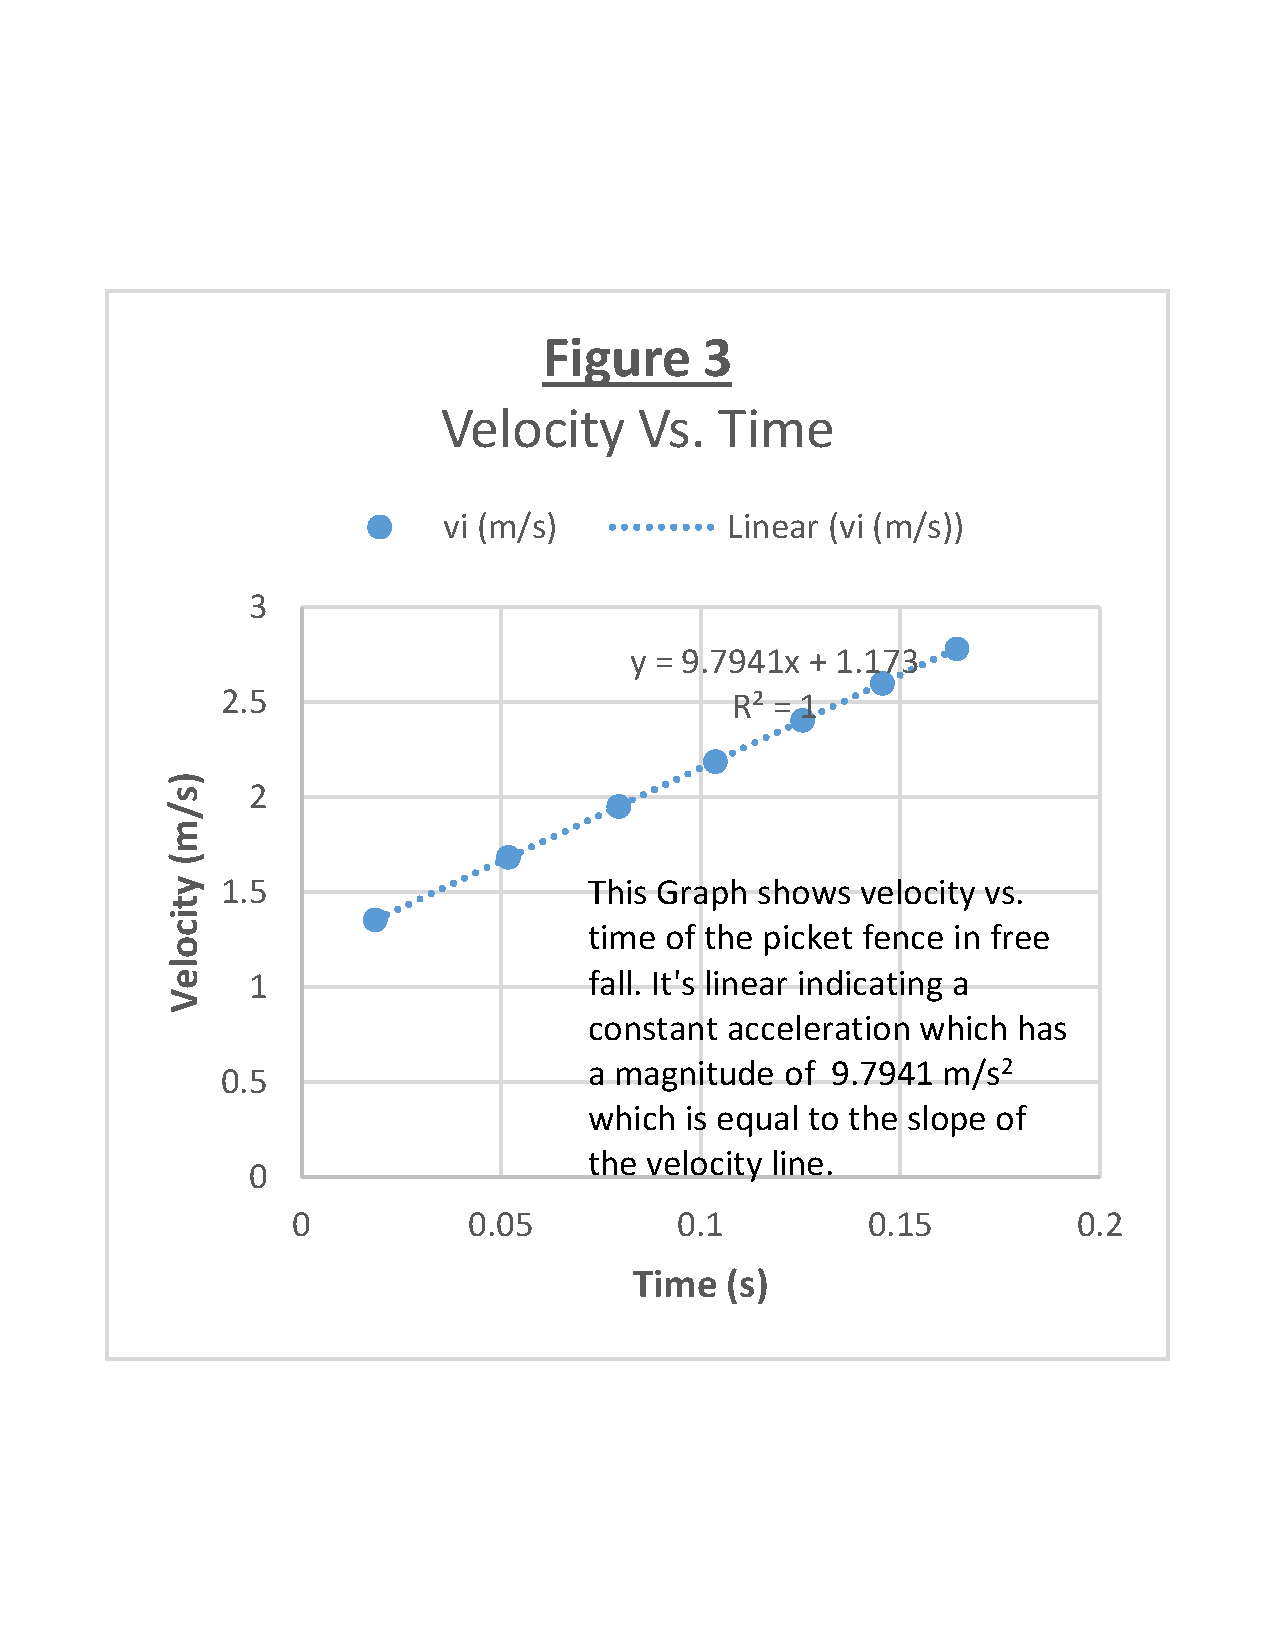
\includegraphics[width=3.5in]{VelocityVsTimeGraph.pdf}
\end{center} 

The slope of the linear regression was 9.7941$\frac{m}{s^2}$ which is the estimated value for acceleration in this experiment. Which makes sense because we know that the acceleration due to gravity is 9.8$\frac{m}{s^2}$, and this is close to our estimated acceleration. Our $R^2$ value was exactly 1 which indicates a perfect straight line.

When calculating the percent error of our actual versus the theoretical, it's necessary to use the equation:

$$percent\hspace{1mm}error = \frac{|actual - theoretical|}{theoretical}*100\%$$

The "theoretical" value is gravity or 9.8$\frac{m}{s^2}$, and the "actual" is the slope our linear regression line from the Velocity vs. Time graph which was 9.7941$\frac{m}{s^2}$.

$$percent\hspace{1mm}error = \frac{|9.7941\frac{m}{s^2} - 9.8\frac{m}{s^2}|}{9.8\frac{m}{s^2}}*100\% = \boxed{.06\%}$$

\subsection{Acceleration-Time Calculations} 

It's necessary to estimate the instantaneous acceleration because we don't have an equation to derive to obtain the instantaneous acceleration. The average acceleration can be calculated by using the equation $\bar{a_i}=\frac{v_i-v_{i-1}}{t_{vi}-t_{v(i-1)}}$. As with velocity, we say that each value for acceleration corresponds to the instant halfway between the two instances of time $t_{vi}$ and $t_{v(i-1)}$ which can be calculated with the equation $t_{ai}=\frac{1}{2}(t_{vi}+t_{v(i-1)})$. The number of average acceleration will be one less then the amount of average velocities, for the same reason the average velocity had one less than the displacement; and this is because we don't know the behavior of the motion prior to the first instant that the photogate collects the data. This means that we don't have a time before the initial time collected by the photo gate to calculate the average velocity between that interval, and this is the same reason average acceleration has one less value than velocity. 

Column J held the times that correspond to the acceleration, so in cell J9 we placed the heading $t_{ai} (s)$. Column K held the average acceleration values, so in cell K9 we placed the heading $a_i (m/s^2)$. In J12 we began doing the calculations for the times corresponding to acceleration, so the equation placed in J12 was "=\textbf{0.5*(G12+G11)}" or $t_{a1}=\frac{1}{2}(t_{v1}+t_{v0})$; then we copied the equation down to cell J17. In K12 we placed the equation "=\textbf{(H12-H11)/(G12-G11)}" or $a_2=\frac{v_2-v_1}{t_{v2}-t_{v1}}$to calculate the average acceleration, we copied this equation down column K to cell K17. 

It's important to keep track of the estimated acceleration that we found by looking at the slope of the linear regression in our veloctiy vs. time graph, so in L9 we place the heading $a_{est} (m/s^2)$. In cells L12 to L17, we placed the estimated acceleration which was 9.7941$\frac{m}{s^2}$. We keep the same values throughout column L, so that we ca n create a nice horizontal line in the acceleration vs. time graph. Then we created the Acceleration vs. time graph by highlighting the values in column J,K, and L and creating another scatter chart with only data points. We then moved the acceleration vs. time graph into a new sheet by clicking on the graph and going to the "Design" tab and clicking "Move Chart" onto a "New Sheet," we named this new sheet: \textbf{AccelGraph}. Once the graph was moved to a new sheet, we gave the graph a title, axis titles, and a appropriate caption. We manipulated the minimum value on the y-axis of our acceleration vs. time graph by right-clicking the y-axis and going to "Format Axis" and then changing the "Minimum" value to zero.  

To create a horizontal line through the $a_{est}$ values, we right-clicked on one of the data points for $a_{est}$ and then selected "Format Data Series." Under the "Line" tab, we selected Automatic, to automatically link all of data points corresponding to that data series. Then we removed the data points for $a_{est}$ by removing the marker for the data series. We then typed out name on the acceleration vs. time graph and on the general spreadsheet. We carefully looked over all of our graphs and data to make sure that they all agree with each other. The spreadsheet and acceleration graph is stapled along with this report. 






\section{Discussion} 

Understanding the machinations of Excel makes manipulating data easy. Excel is a great program to organize data and create appropriate graphs, we can use Excel to organize and manipulate data in future experiments as well as create nice graphs. Excel has a plethora of fuctions that make organizing and manipulating data easy and neat, for example the function to create a linear regression allowed us to quickly obtain the estimated acceleration from the velocity vs. time graph.    



\section{References}

\hspace{-6.5mm}
Introduction to Data Analysis on Excel Physics 06 Lab, Dr. Melanie Lutz\\



\end{document}
